This section specifies the software architecture requirements and the software
architecture design at the second level of granularity - the management service
of the benchmarking system. The management service will be responsible for all
administration of results, test data, user management. The management service
will further integrate with the client watcher application which will be uesd to
benchmark the user uploaded applications.

\section{Overall Software Architecture}
\subsection{Architecture Requirements}
This section discusses the software architecture requirements around the
backend management system infrastructure. The backend management system will be
responsible for the delegation of jobs to cluster nodes, persisting of results,
user management and allowing users to derive value from reporting. In particular
the architecture requirements at the second level of granularity is specified.

The architecture requirements should specify:
\begin{itemize}
	\item the architectural responsibilities which need to be addressed
	\item the access and integration requirements for the system
	\item the quality requirements
\end{itemize}

Figure \ref{fig:managementInfrastructure} show the a high-level infrastructure
view of the Management service.

\begin{figure}[H]
  \begin{center}
  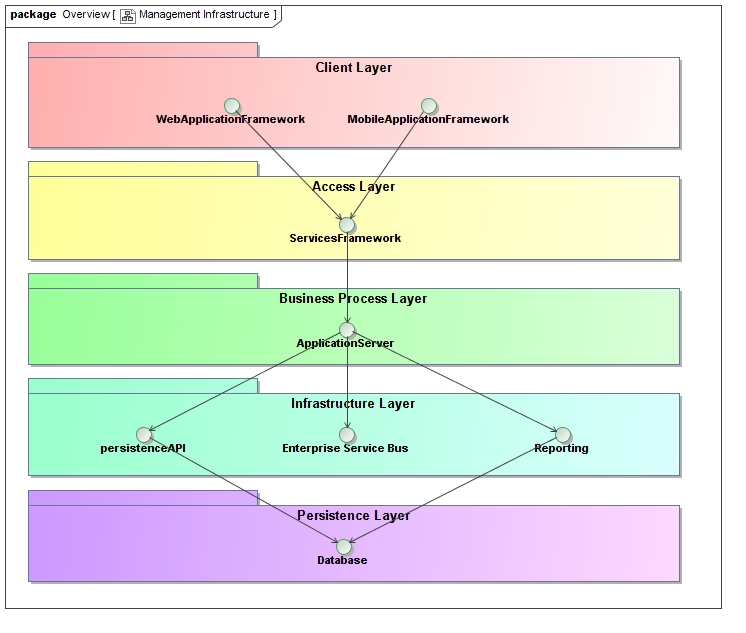
\includegraphics[scale=0.4]{../Diagrams and Charts/Overview/ManagementInfrastructure.jpg}
  \caption{A high-level overview of the software architecture for the Management Service}
  \label{fig:managementInfrastructure}
  \end{center}
\end{figure}


\subsubsection{Access and Integration Requirements}
\label{sec:accessIntegrationRequirementsManagementSystem}
\paragraph{Access Channels}
The access channels can be divided into two broard categories based on the user type
\begin{itemize}
	\item Human Access Channel
	\item System Access Channel
\end{itemize}

\subparagraph{Human Access Channel}
\label{sec:humanAccessChannelManagementSystem}
The system will be providing a REST based access channel to be used by human
users. The two interfacing applications to be delivered are
\begin{itemize}
	\item HTML 5/JavaScript Single Page Application Web Interface
	\item Mobile Applications
\end{itemize}

\subparagraph{System Access Channel}
The system will expose a further access channel to be used by the so-called
"Benchmark Client" or "wacther" application. This access channel will be
utilizing a message bus architecture to deliver messages between the client
and the management backend system.

This access channel will however not be accessable to end users.

\paragraph{Integration Channels}
The various integration channels of the benchmarking system
\begin{itemize}
	\item Integration with a persistence provider
	\item Integration with the human access channels, such as web and
		mobile interfaces 
	\item Integration with the message bus architecture
	\item Integration with Linux Containers
\end{itemize}

The integration with the persistence provider is required as we need to persist
the measurements obtained with the benchmarking client. Further more as per the
client's request, test data must also be persisted as it is envision that a
repository of test data will be build.

In order to make the results from the benchmarking tests useful, users will
need some way to interact and manipulate the data in order to be able to
derive value from this data. To enable users to interact with the data,
two human access channels will be created, namely a web and mobile interface
to allow users to interact and derive value from the data.

The final intergration required by the management system is that of integration
with the message bus. In order to better decouple the benchmarking client and
management systems, a message bus architecture was introduced. The management
system will process the results from a queue structure managed by the messaging
system. 

Once a program is uploaded via the a human access channel, it will be deployed
to the benchmarking cluster in a Linux Container (LXC), upon which the
benchmarking will commence.  The reason for utilizing Linux containers is in
order to meet the security quality requirements as provided in
section \ref{sec:securityQualityRequirement}.

\subsubsection{Quality Requirements}
\label{sec:qualityRequirementManagementSystem}
The quality requirement are the requirements around the quality attributes of
the systems and the services it provides. This includes requirements like
maintainability, flexibility, extensibility, performance, scalability, security,
auditability, usability and testability requirements.
\paragraph{Security}
\label{sec:securityQualityRequirement}
\paragraph{Authentication}
The system needs to support a simple registration and authentication framework
which will determine what each user can do based on their authority level. This
also involves users at a higher level of authority having the ability to manage
the users at a level of authority lower than theirs.
\paragraph{Flexibility}
Persistence architectures and reporting infrastructures are rapidly evolving as can
be seen from the rapid growth of NoSQL databases, semantic knowledge repositories and big data
stores. In this context it is important that the application functionality is not locked into any
specific persistence technology and that one is able to easily modify the persistence provider and
reporting framework.\\
Futhermore it is important that the Client layer can easily be swapped out for a different
layer that accesses the system in a different why using the layer beneath it.
\paragraph{Maintainability}
Amongst the most important quality requirements for the system is
maintainability. It should be easy to maintain the system in the future. To this end

\begin{itemize}
\item future developers should be able to easily understand the system,
\item the technologies chosen for the system an be reasonably expected to be available for a long
time,
\item and developers should be able to easily and relatively quickly
	\begin{itemize}
		\item change aspects of the functionality the system provides, and
		\item add new functionality to the system.
	\end{itemize}
\item it should be easy to modify reports and add reports new reports to the system.
\end{itemize}

\paragraph{Scalability}
The system needs to be able to handle high amounts of concurrent traffic.
In addition to this the system should also be protected against
denial of service attacks why the way the system handels concurrent traffic.

\paragraph{Testability}
All services offered by the system must be testable through
\begin{enumerate}
	\item automated unit tests testing components in isolation using mock objects, and
	\item automated integration tests where components are integrated within the actual environment.
\end{enumerate}

In either case, these functional tests should verify that
\begin{itemize}
	\item the service is provided if all pre-conditions are met (i.e. that no exception is raised)
	\item the correct execption is throw when the corresponding pre-condition
	is violated.
	\item that all post-conditions hold true once the service has been provided.
\end{itemize}

In addition to functional testing, the quality requirements should also be tested.

\paragraph{Usability}
The system should be intuitive and efficient to use. Computer literacy can be
assumed, but the goal of the system is to be an easy to use Benchmarking
Service that does not require complex configuration. As such users should
not experience much difficulty in using the interface. Error messages should
also be self-explanatory.

\paragraph{Integrability}
The system should be able to easily address future integration requirements
by providing access to its services using widely adopted public standards.
All use cases which are available to human users should also be accessible from external systems.

\paragraph{Deployability}
\label{sec:systemDeployability}

\subsubsection{Architectural Responsibilities}
\begin{figure}[H]
	\begin{center}
	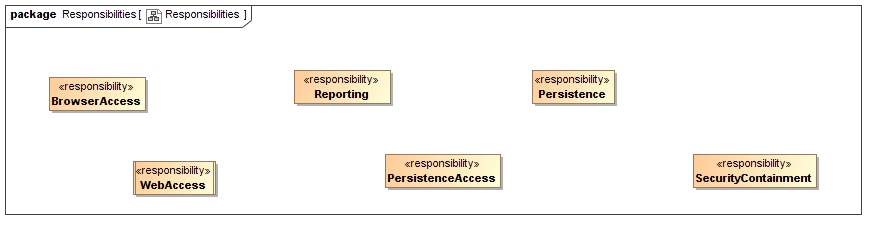
\includegraphics[scale=0.5]{../Diagrams and Charts/Architecture/Responsibilities.jpg}
	\caption{A high-level overview of the software architecture responsibilities}
	\end{center}
	\label{fig:architectureResponsibilities}
\end{figure}

The figure \ref{fig:architectureResponsibilities} shows the allocation of architectural
responsibilities to architectural components. The system requires an execution environment
in which the business processes realizing these services can be executed in. Further more,
system has two human channels, allowing human users to access the system via a  web interface
or mobile device. Furthermore the system requires a persistence interface which abstracts the
underlying persistence provider. The management system has one system channel, which is used
to allow for integration with the watcher applications running on cluster nodes.


\subsection{Architecture Design}
This section specifies a very high-level software architecture design, i.e.
the software architecture design for the second level of granularity. It
includes the allocation of architectural responsibilities to architectural
components, any tactics which should be used at the current level of
granularity to address quality requirements,

\subsubsection{Tactics}
At this high level of abstraction, we do not specify any architectural tactics
in order to concretely address the quality requirements for the system.

\subsubsection{Architectural Components}
Figure \ref{fig:architectureResponsibilityAllocation} shows the allocation of
architectural responsibilities to architectural components. 
\begin{figure}[H]
	\begin{center}
	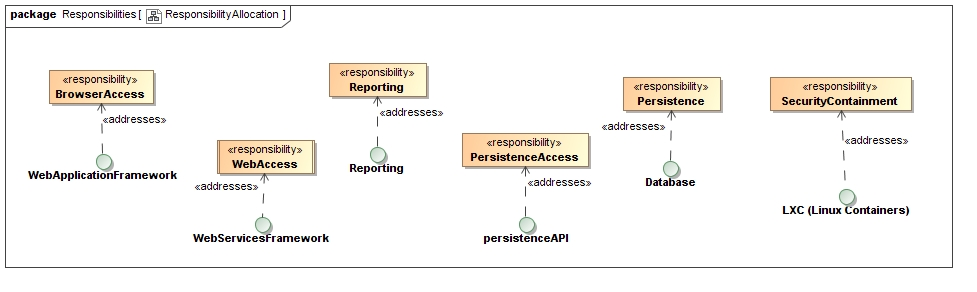
\includegraphics[scale=0.5]{../Diagrams and Charts/Architecture/ResponsibilityAllocation.jpg}
	\caption{The abstract architectural components to which the architectural responsibilities are
assigned.}
	\end{center}
	\label{fig:architectureResponsibilityAllocation}
\end{figure}

\section{Database}
The database is a persistence provider providing long term, organized storage
of the data which will be generated through the application. Various types of
database exist, which are mainly categorized based on the approach with which
the provider in questions represents and stores the data internally. Some of 
the types of databases which where considered for this project include
\begin{itemize}
	\item Relational Databases e.g. MySQL, PostgreSQL
	\item Document-oriented Databases e.g. MongoDB, Couchbase
	\item Graph-based Databases Neo4j, OrientDB
\end{itemize}

In choosing a persistence provider, it is important to consider the data as
well as the relationship between the data to ensure the correct type of 
provider is selected.

The data to be generated by the benchmarking service will have a very flat
relationship structure between data elememtns. This flat structure naturally
makes the data well suited for a document-based persistence provider.

\subsection{Architecture Requirements}
\subsubsection{Access and Integration Requirements}
\subsubsection{Quality Requirements}
\paragraph{Scalability}
The database selected must allow for horizontal scaling of the infrastructure,
which means that the database should be able to scale across different hosts to
form a combined and intelligant cluster. Optional support of distribution the
database across providers will be benefical for future expansion.

\paragraph{Performance}
As the database will receive a higher ratio of reading to writing operations
per sec, this must be kept in mind when selecting the required database. The
database should also be able to deliver on strict Service Level Agreements
(SLA), especially on availability.

\paragraph{Reliability}
As the database will be used to build a repository of knowledge, in the form of
historical benchmark results and test data sets, it is of the utmost importance
that the selected database store is able to preserve data reliably even in the
event of a possible disaster. The one again highlights the need for a database
store which is able to function across data centers.

\paragraph{Integrability}
The chosen database should be supporte by the chosen perisistence API realization
in such a way, that from the business logic, there are no database specific
code. The chosen persistence API was chosen for this exact reason as to support
the swapping out of the underlying database store without the need to change any
higher level code. As not all databases are supported by the persistence API,
this places an inherit technological constraint on the database stores which can
be utilized in the project.

\paragraph{Deployability}
This requirement places no further restrictions on the requirements as set out
in section \ref{sec:systemDeployability}.

\subsubsection{Architectural Responsibilities}
The architectural responsibilities of the database are shown in 
Figure \ref{fig:databaseResponsibilities}
\begin{figure}[H]
	\begin{center}
	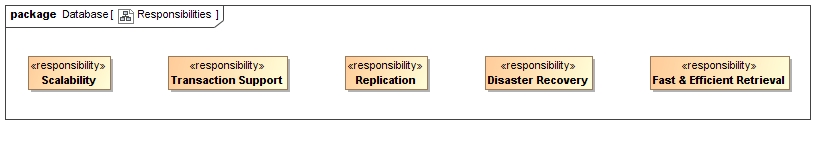
\includegraphics[scale=0.5]{../Diagrams and Charts/Database/Responsibilities.jpg}
	\caption{The architectural responsibilities of the Database}
	\label{fig:databaseResponsibilities}
	\end{center}
\end{figure}

\subsubsection{Architecture Constraints}
\subsection{Architecture Design}
\subsubsection{Tactics}
Tactics which should be used by the database to address the quality requirements:
\begin{itemize}
	\item \textit{Scaling out resources} to allow for flexiable and cheap
		improvement in performance and scalability.
	\item \textit{Efficient Persistence} to allow for the quick and efficient
		retrieval of data from the provider aiding in performance
		improvement.
	\item \textit{Efficient Storage Usage} to minimize the required
	infrastructure needed by the service.
	\item \textit{Spread Load} in order to fulfill the required scalability
		and performance requirements as set out above.
	\item \textit{Removing single points of failure} to ensure data is
		protected against disasters as the client will be building a
		knowledge repository.
\end{itemize}
\subsubsection{Architectural Components}
\subsubsection{Frameworks and Technologies}
\paragraph{Concrete Realization of Architectural Components}
\paragraph{Tactics}
\paragraph{Tools}
\paragraph{Concepts and Constraints for Application Components}

\section{Persistence API}
The persistence API provides abstracted access to a persistence provider while
remaing decoupled from the underlying technology, including but not limited to
database, SQL version and transaction management, whilst employing a range of
software engineering tactics to concretely address required quality
requirements required for the persistence domain.

\subsection{Architecture Requirements}
The architectural requirements for the persistence API include the refined
quality requirements and architectural requirements listed below. The
architectural constraints for this lower level components are the same as for
the system as whole, as referred to in
section \ref{sec:systemArchitecturalConstraints} with further extensions as
specified in section \ref{sec:persistenceAPIArchitecturalConstraints}.

\subsubsection{Quality Requirements}
\paragraph{Flexibility}
The provided persistence API should be able to adapt to the rapidly evolving
persistence architecture domain, especially in terms of the different
methodologies of storing data such as relational and NoSQL data stores. It is
further import that the persistence layer is not locked to any specific
persistence technology.

Further the chosen API should to force the use of any vendor specific
transaction management, but should rather provide an abstraction layer allowing
the use of any transaction manager implementing the required interface.

\paragraph{Maintainability}
\label{sec:persistenceAPIMaintainability}
The used persistence API should be in a mature stage of the software development
life cycle as to guard against a rapidly evolving changing API. The chosen
persistence API should be an open standard with multiple realization as to guard
against realization technologies be abandoned. This will allow in future an easier
switch to another persistence API implementation if required for the long term
maintance and use of the project.

\paragraph{Scalability}
The chosen persistence API should be able to allow for future scaling of the
infrastructure either horizontally or vertically with a preference for
horizontal scaling.

\paragraph{Performance}
The persistence API should allow for the use of certain architectural tactics
to increase performance. Specifically the following tactics should be supported
to some extent
\begin{itemize}
	\item Object Caching
	\item Connection Pooling
	\item Thread Provisioning
	\item Scheduling
\end{itemize}

\paragraph{Reliability}
The chosen API should allow security at least providing authorization on
entities managed by the underlying persistence technology architecture.

\subsubsection{Architectural Responsibilities}
The architectural responsibilities of the persistence API are shown in
Figure \ref{fig:persistenceResponsibilities}
\begin{figure}[H]
	\begin{center}
	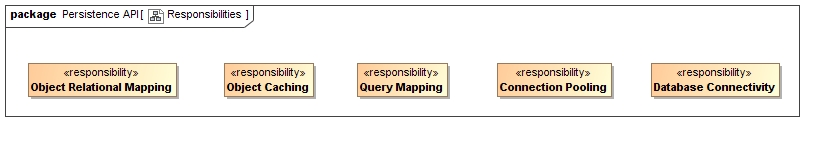
\includegraphics[scale=0.5]{../Diagrams and Charts/Persistence API/Responsibilities.jpg}
	\caption{The architectural responsibilities of the Persistence API}
	\label{fig:persistenceResponsibilities}
	\end{center}
\end{figure}

\subsubsection{Architecture Constraints}
The chosen persistence API should be a currently active standard, with a medium
to large sized active community supporting the standard and should be realized
by at least three active realizations of the chosen API as to ensure future
maintainability as set out by the required quality requirement in
section \ref{sec:persistenceAPIMaintainability}.
\label{sec:persistenceAPIArchitecturalConstraints}

\subsection{Architecture Design}
\subsubsection{Tactics}
The persistence API implement the following tactics:
\begin{itemize}
	\item \textit{Object Relational Mapping} to reduce code bulk, improve
		maintainability and allow for decoupling from the persistence
		provider.
	\item \textit{Query Mapping} from queries across a graph of Java objects
		onto the database queries used in the selected database
		technology and provider.
	\item \textit{Object caching} to improve scalability and performance.
	\item \textit{Transactions} with 2-phase commit to improve reliability
		of processes.
	\item \textit{Transaction Neutral API} allow the use of any transaction manager
		implementing the required interface as to improve flexibility and
		future maintainability.
	\item \textit{Connection Pooling} to improve performance and scalability.
\end{itemize}

\subsubsection{Architectural Components}
The architectural components of the persistence API are shown in Figure \ref{fig:persistenceResponsibilityAllocation}
\begin{figure}[H]
	\begin{center}
	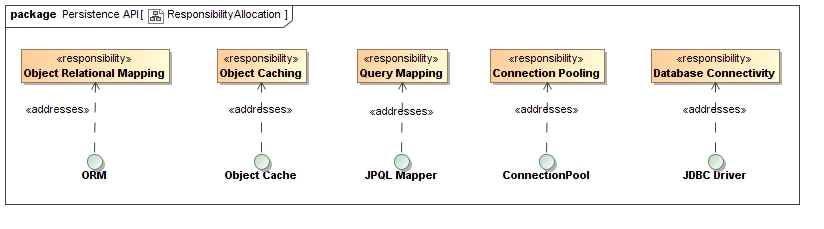
\includegraphics[scale=0.5]{../Diagrams and Charts/Persistence API/ResponsibilityAllocation.jpg}
	\caption{The abstract components to which the architectural responsibilities are assigned.}
	\label{fig:persistenceResponsibilityAllocation}
	\end{center}
\end{figure}

\subsubsection{Frameworks and Technologies}
A JPA 2.1 (Java Persistence API Version 2.1) provider will be used as a
persistence API. The chosen concrete implementation used will be Hibernate as
it has support for both relational and NoSQL persistence providers.

The JPA 2.1 API is a widely supported public standard which are implemented by
the following products:
\begin{itemize}
	\item Hibernate
	\item EclipseLink
	\item DataNucleus
\end{itemize}

Further more the listed implementations all support the use of NoSQL databases
by utilizing the JPA standard for relational databases. Thus the required
quality requirements of using an open standard with multiple implementations
supporting both relational and NoSQL database are fulfilled.

The persistence context (EntityManager) will will be dependency injected into
services requiring access to persistent data. JPA providers do implement
\begin{itemize}
	\item \textit{Object Relational Mapping} including the mapping of
		relationships between objects via a provided ORM
		implementation such as Hibernate or EclipseLink.
	\item \textit{Query Mapping} from object-oriented queries across the
		domain object graph to queries for a specific database provider.
	\item \textit{Object caching} within the persistence context with
		in-memory or NoSQL database based caching allow for the
		fulfilment of the performance, flexibility and scalability
		quality requirements.
	\item \textit{Transactions} are supported through the use of the \textit{Java Transaction API (JTA)}.
	\item \textit{Transaction Neutral API} is supported through the Spring
		Framework transaction manager supporting a consistent programming
		model across different transaction APIs such as
		Java Transaction API, JDBC, Hibernate, Java Persistence API and
		Java Data Objects.
	\item \textit{Connection Pooling} is provided through a JCA connector
		based implementation of a JDBC driver.
\end{itemize}

Queries will be specified as Spring Data JPA queries, thereby reducing
boilerplate code which ease future maintenance and development, as the queries
are not specific to any underlying query language e.g. SQL or any underlying
persistence technology such as relational or NoSQL providers.

\paragraph{Concepts and Constraints for Application Components}
The application concepts within the persistence domain include
\begin{itemize}
	\item \textit{Domain objects} which host long-living state objects, and is realized in the Java architecture as Plain Old Java Objects (POJO's) which doesn't contain any business logic.
	\item \textit{Queries across object graph of domain objects} through which the required information of state in the domain objects is retrieved, modified and removed.
\end{itemize}

\section{Web Services Framework}
The web services framework is used to expose business services in a
technology-neutral way over some network, which in most cases is the public
Internet.  Wrapping business services in a technology-neutral layer allows
one to decouple the front-end technologies, specifically the user interface
technologies from the back-end technologies, while simultaneously allowing for the decoupling
of back-end services from one another, in effect communication between disparate
applications.  This decoupling provides one with the ability to vary either the
front-end technologies and back-end technologies independently from one
another.  Furthermore this allows one to write back-end services in the most
appropriate technology stack and then have seamless communication between these
individual components.

\subsection{Architecture Requirements}
The architectural requirements for the web service framework include the
refined quality requirements and architectural requirements listed below. The
architectural constraints for this lower level components are the same as for
the system as whole, as referred to in section \ref{sec:systemArchitecturalConstraints}
with further extensions as specified in section \ref{sec:persistenceAPIArchitecturalConstraints}.

\subsubsection{Access and Integration Requirements}
\subsubsection{Quality Requirements}
\paragraph{Maintainability}
\label{sec:webServicesFrameworkMaintainability}
The web services framework is concerned with wrapping business logic, thereby
allowing one to categorize this as so called "plumbing code" which should be as
far as possible be removed from the actual code. This code is normally applied
by the use of annotations in the Java context or by weaving the code into
existing business code using aspects.

Using the above mentioned approach allows one more easily to maintain the code
base.

\paragraph{Integrability}
The framework should enable one to expose business services in a technology
neutral way to allow for easy integration with other independent business
services and systems.  The chosen technology neutral format should be supported
by the business services and system that require integration.

\subsubsection{Architectural Responsibilities}
The architectural responsibilities of the Web Services Framework are shown in 
Figure \ref{fig:webServicesFrameworkResponsibilities}
\begin{figure}[H]
	\begin{center}
	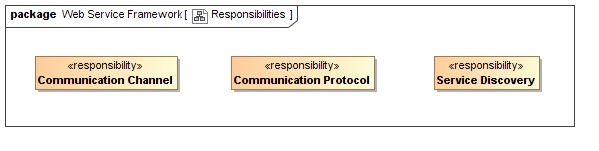
\includegraphics[scale=0.5]{../Diagrams and Charts/Web Services Framework/Responsibilities.jpg}
	\caption{The architectural responsibilities of the Web Services Framework}
	\label{fig:webServicesFrameworkResponsibilities}
	\end{center}
\end{figure}

\subsubsection{Architecture Constraints}
The chosen persistence API should be a currently active standard, with a medium
to large sized active community supporting the standard and should be realized
by at least three active realizations of the chosen API as to ensure future 
maintainability as stout by the required quality requirement in 
section \ref{sec:webServicesFrameworkMaintainability}.

\subsection{Architecture Design}
\subsubsection{Tactics}
The Web Services Framework implement the following tactics:
\paragraph{Support Communication Channels}
The web services framework should support the communication channel to be used
between the client and server as well as between between business services.
With regards to this project the communication channels will consists of a
standards based network connection between all parties, with the communication
channel not necessarily being uniform between all parties. The most likely
communication channel between the client and server will be the Internet
network with a internet network between business services.

\paragraph{Support Standard Communication Protocols}
The web service framework should support standards based communication
protocols as this will ensure the highest change of ensuring full
integrability between client and other business services. All parties should
at least support one of the standards the selected web services framework
supports, thereby ensuring all parties will have successful communication.

\paragraph{Dynamic Service Discovery}
The provided web services framework should allow for dynamic service discovery
by the clients with the clients only knowing where to locate the root service.
This will ensure easier maintainability as clients and other services will not
need to be informed with the location of the services have changed.

\subsubsection{Architectural Components}
The architectural components of the Web Services Framework are shown in Figure \ref{fig:webServicesFrameworkResponsibilityAllocation}
\begin{figure}[H]
	\begin{center}
	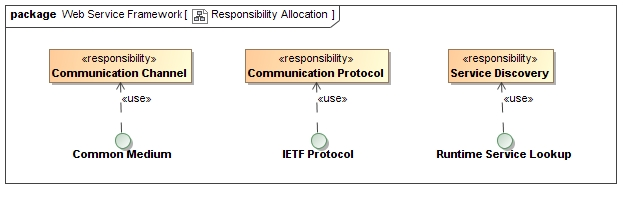
\includegraphics[scale=0.5]{../Diagrams and Charts/Web Services Framework/ResponsibilityAllocation.jpg}
	\caption{The abstract components to which the Web Services Framework responsibilities are assigned.}
	\label{fig:webServicesFrameworkResponsibilityAllocation}
	\end{center}
\end{figure}

\subsubsection{Frameworks and Technologies}
\paragraph{Concrete Realization of Architectural Components}
The concrete components addressing the required responsibilities are shown in Figure \ref{ref:webServicesFrameworkResponsibilityRealization}.
\begin{figure}[H]
	\begin{center}
	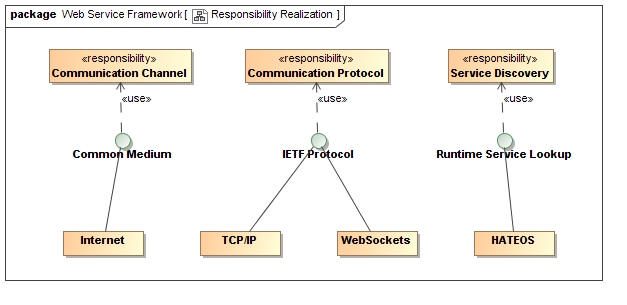
\includegraphics[scale=0.5]{../Diagrams and Charts/Web Services Framework/ResponsibilityRealization.jpg}
	\caption{The components within Jersey addressing the architectural responsibilities of the Web Services Framework}
	\label{fig:webServicesFrameworkResponsibilityRealization}
	\end{center}
\end{figure}

\section{Web Application Framework}
This section specifies the software architecture requirements and the software
architecture design for web application framework.

\subsection{Architecture Requirements}
The web application framework provides the software architecture for the software
providing browser based access to human users.

\subsubsection{Access and Integration Requirements}
The web application must be usable by humans using any standards compliant web
browser. The system should be usable by the latest versions of the Mozilla 
Firefox, Chrome, Safari, Opera and Internet Explorer. The web
application will need to integrate with the services/business processes layer
via a REST API.

\subsubsection{Quality Requirements}
The most important quality requirements for the web application layer are
\begin{itemize}
	\item Usability
	\item Maintainability
	\item Flexibility
	\item Performance
\end{itemize}
	
\subsubsection{Architectural Responsibilities}
The architectural responsibilities of the Web Application Framework are shown in 
Figure \ref{fig:webApplicationFrameworkResponsibilities}
\begin{figure}[H]
	\begin{center}
	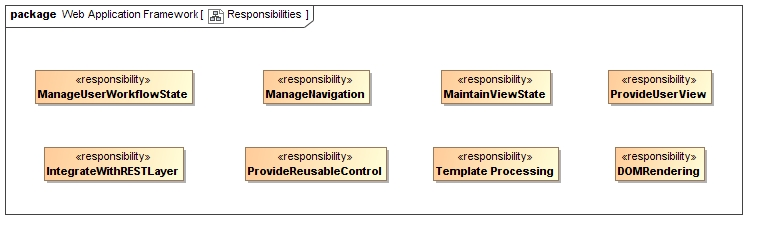
\includegraphics[scale=0.35]{../Diagrams and Charts/Web Application Framework/Responsibilities.jpg}
	\caption{The architectural responsibilities of the Web Application Framework}
	\label{fig:webApplicationFrameworkResponsibilities}
	\end{center}
\end{figure}

\subsubsection{Architecture Constraints}
The architectural constraints of the system are propagated directly to all 
components including the web application framework. It must hence be open source
and make use of public standards. The chosen technology should also be well 
supported and documented and allow for possible mobile integration.

\subsection{Architecture Design}
This section specifies the very high-level software architecture design, i.e.
the software architecture design for the top level of granularity. Including 
allocation of architectural responsibilities to architectural components, any
tactics which should be used at the current level of granularity to address
quality requirements.

\subsubsection{Tactics}
Tactics which should be used to address the quality requirements should include:
\begin{itemize}
	\item caching of pre-generated and pre-populated HTML pages for performance
	\item virtual DOM for in-memory updates, incremental builds and efficient 
	diffing based on differentiation between static and dynamic DOM elements
\end{itemize}
\subsubsection{Architectural Components}
The architectural components of the  Web Application Framework are shown in Figure \ref{fig:webApplicationFrameworkResponsibilityAllocation}
\begin{figure}[H]
	\begin{center}
	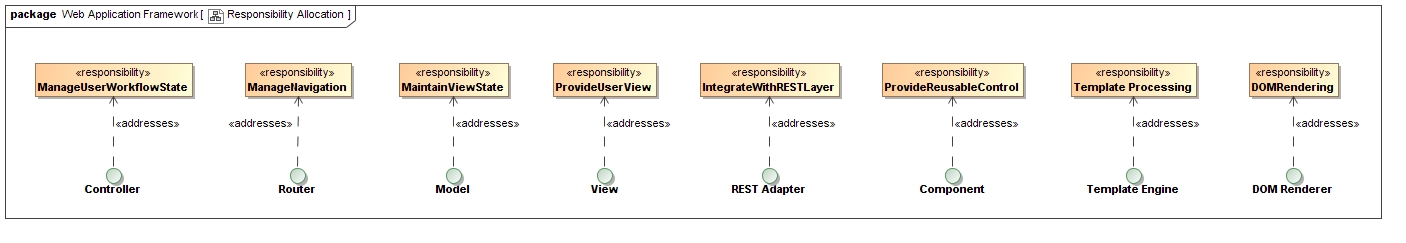
\includegraphics[scale=0.35]{../Diagrams and Charts/Web Application Framework/ResponsibilityAllocation.jpg}
	\caption{The abstract components to which the Web Application Framework responsibilities are assigned.}
	\label{fig:webApplicationFrameworkResponsibilityAllocation}
	\end{center}
\end{figure}

\subsubsection{Frameworks and Technologies}
The web framework will be based on \textbf{ReactJS}. ReactJS is an open-source web
application framework. The framework promises a model in which sub-components
cannot directly affect enclosing components.

Core reasons for using ReactJS:
\begin{itemize}
	\item The framework requires a defined structure which aids in maintainability.
	\item The framework is maintained not only by a community of users but also
	by Facebook and Instagram, this aids further in maintainability due to the 
	constant upkeep of documentation.
	\item The model supports integration with RESTful API services.
	\item Release of React Native which will allow for React based architecture 
	to native Android and iOS applications making the task of developing an 
	application, should time permit, easier.
\end{itemize}
Other frameworks were considered;
\textbf{AngularJS}: which is a powerful extensible framework with good modularization
, however, there is no consistent way to approach application development which may 
lead to difficulty regarding maintenance. The virtual DOM approach in ReactJS is more
efficient. Angular is also being replaced by ReactJS as the current standard for web 
application development and as a team with minimal experience in Angular we decided 
that we'd rather get experience in a future standard which is also easier to learn.

\paragraph{Concrete Realization of Architectural Components}
The concrete realization of components within \textbf{ReactJS} are shown in Figure
\paragraph{Tactics}
\paragraph{Tools}
\begin{itemize}
	\item Uses JavaScript so no need to learn another language/syntax.
\end{itemize}
\paragraph{Concepts and Constraints for Application Components}

\section{Reporting}
The Reporting Module provides functionality to generate and compare reports
of single/or multiple benchmarks, with the option to export them as csv,
whilst still complying with the quality requirements defined for the system.

\subsection{Architecture Requirements}
\subsubsection{Quality Requirements}
\paragraph*{Flexibility}
The reporting module should be flexible enough to add different elements,
such as graphs, charts and tables. The color scheme should also be easily
changed.

\paragraph*{Performance}
The performance of the reports should as minimalistic as possible, such that the
page is responsive as possible.

\paragraph*{Reliability}
Each report must be reliable with the data it represents, as this is what the
user will be referring to.



\subsection{Architecture Design}
\subsubsection{Architectural Responsibilities, Components and Realization}
The architectural components of the Reporting Module are shown in Figure \ref{fig:reportingResponsibilityAllocation}
\begin{figure}[H]
	\begin{center}
	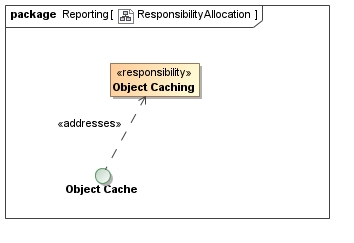
\includegraphics[scale=0.5]{../Diagrams and Charts/Reporting/ResponsibilityAllocation.jpg}
	\caption{The abstract components to which the architectural responsibilities are assigned.}
	\label{fig:reportingResponsibilityAllocation}
	\end{center}
\end{figure}



\subsubsection{Tactics}
The Reporting module should implement the following tactics:
\begin{itemize}
  \item \textit{Report caching} to improve scalability and performance.
\end{itemize}



\subsubsection{Frameworks and Technologies}
The frameworks and technologies used for reporting will consist of JavaScript,
HTML and CSS. With the exporting of reports using a JavaScript library called jsPDF.

We have considered using the jasper reports to generate reports, but it does
 not provide the full functionality that we are looking for. Such as exporting the graphics of the reports.

